\hypertarget{interface_t_p_chart_basic}{
\section{TPChartBasic Class Reference}
\label{interface_t_p_chart_basic}\index{TPChartBasic@{TPChartBasic}}
}
{\tt \#import $<$TPChartBasic.h$>$}

Inheritance diagram for TPChartBasic::\begin{figure}[H]
\begin{center}
\leavevmode
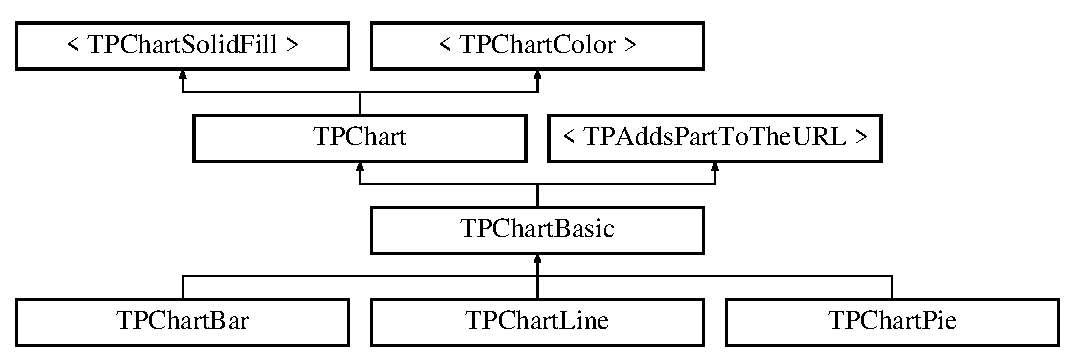
\includegraphics[height=4cm]{interface_t_p_chart_basic}
\end{center}
\end{figure}
\subsection*{Public Member Functions}
\begin{CompactItemize}
\item 
(NSInteger) - \hyperlink{interface_t_p_chart_basic_a41306abeba81e4799c5b45eff1fefea}{addNewLine:}
\item 
(NSArray $\ast$) - \hyperlink{interface_t_p_chart_basic_55444751da9bebff034548c8a8c9c05a}{valuesForRow:}
\item 
(NSInteger) - \hyperlink{interface_t_p_chart_basic_dbaf4e508385b4d2b56ff1c5b26fa518}{addNewRowTitle:}
\item 
(void) - \hyperlink{interface_t_p_chart_basic_ac52ed925271b579ff3ec12835ed4179}{setRowTitle:withId:}
\item 
(void) - \hyperlink{interface_t_p_chart_basic_a60b292eef70dacf23030a75f4fd0dd8}{setRowTtiles:}
\item 
(NSString $\ast$) - \hyperlink{interface_t_p_chart_basic_29c20cc728ebf4bca74d1cc0acc51841}{titleForRow:}
\end{CompactItemize}


\subsection{Detailed Description}
The super class for the basic charts: Bar,Pie,Line Has mutliple list of values and each list has a name/title 

\subsection{Member Function Documentation}
\hypertarget{interface_t_p_chart_basic_a41306abeba81e4799c5b45eff1fefea}{
\index{TPChartBasic@{TPChartBasic}!addNewLine:@{addNewLine:}}
\index{addNewLine:@{addNewLine:}!TPChartBasic@{TPChartBasic}}
\subsubsection[{addNewLine:}]{\setlength{\rightskip}{0pt plus 5cm}- (NSInteger) addNewLine: (NSArray $\ast$) {\em rowValues}}}
\label{interface_t_p_chart_basic_a41306abeba81e4799c5b45eff1fefea}


Adds a new line of values to the chart \begin{Desc}
\item[Parameters:]
\begin{description}
\item[{\em rowValues}]array with a list of values \end{description}
\end{Desc}
\begin{Desc}
\item[Returns:]index of the added row \end{Desc}
\hypertarget{interface_t_p_chart_basic_dbaf4e508385b4d2b56ff1c5b26fa518}{
\index{TPChartBasic@{TPChartBasic}!addNewRowTitle:@{addNewRowTitle:}}
\index{addNewRowTitle:@{addNewRowTitle:}!TPChartBasic@{TPChartBasic}}
\subsubsection[{addNewRowTitle:}]{\setlength{\rightskip}{0pt plus 5cm}- (NSInteger) addNewRowTitle: (NSString $\ast$) {\em title}}}
\label{interface_t_p_chart_basic_dbaf4e508385b4d2b56ff1c5b26fa518}


Adds a new rowtitle to the chart \begin{Desc}
\item[Parameters:]
\begin{description}
\item[{\em title}]new title to add \end{description}
\end{Desc}
\begin{Desc}
\item[Returns:]index of the new added title; \end{Desc}
\hypertarget{interface_t_p_chart_basic_ac52ed925271b579ff3ec12835ed4179}{
\index{TPChartBasic@{TPChartBasic}!setRowTitle:withId:@{setRowTitle:withId:}}
\index{setRowTitle:withId:@{setRowTitle:withId:}!TPChartBasic@{TPChartBasic}}
\subsubsection[{setRowTitle:withId:}]{\setlength{\rightskip}{0pt plus 5cm}- (void) setRowTitle: (NSString $\ast$) {\em title}\/ withId: (NSInteger) {\em rowId}}}
\label{interface_t_p_chart_basic_ac52ed925271b579ff3ec12835ed4179}


Sets the row title for a specified index \begin{Desc}
\item[Parameters:]
\begin{description}
\item[{\em title}]title to add \item[{\em rowId}]index where the title should be set \end{description}
\end{Desc}
\hypertarget{interface_t_p_chart_basic_a60b292eef70dacf23030a75f4fd0dd8}{
\index{TPChartBasic@{TPChartBasic}!setRowTtiles:@{setRowTtiles:}}
\index{setRowTtiles:@{setRowTtiles:}!TPChartBasic@{TPChartBasic}}
\subsubsection[{setRowTtiles:}]{\setlength{\rightskip}{0pt plus 5cm}- (void) setRowTtiles: (NSArray $\ast$) {\em titles}}}
\label{interface_t_p_chart_basic_a60b292eef70dacf23030a75f4fd0dd8}


set the titles of all rows \begin{Desc}
\item[Parameters:]
\begin{description}
\item[{\em titles}]NSArray with the titles as NSStrings \end{description}
\end{Desc}
\hypertarget{interface_t_p_chart_basic_29c20cc728ebf4bca74d1cc0acc51841}{
\index{TPChartBasic@{TPChartBasic}!titleForRow:@{titleForRow:}}
\index{titleForRow:@{titleForRow:}!TPChartBasic@{TPChartBasic}}
\subsubsection[{titleForRow:}]{\setlength{\rightskip}{0pt plus 5cm}- (NSString $\ast$) titleForRow: (NSInteger) {\em rowId}}}
\label{interface_t_p_chart_basic_29c20cc728ebf4bca74d1cc0acc51841}


Returns the title of the row with the specified index \begin{Desc}
\item[Parameters:]
\begin{description}
\item[{\em rowId}]index of the row \end{description}
\end{Desc}
\begin{Desc}
\item[Returns:]title of the row \end{Desc}
\hypertarget{interface_t_p_chart_basic_55444751da9bebff034548c8a8c9c05a}{
\index{TPChartBasic@{TPChartBasic}!valuesForRow:@{valuesForRow:}}
\index{valuesForRow:@{valuesForRow:}!TPChartBasic@{TPChartBasic}}
\subsubsection[{valuesForRow:}]{\setlength{\rightskip}{0pt plus 5cm}- (NSArray $\ast$) valuesForRow: (NSInteger) {\em rowIndex}}}
\label{interface_t_p_chart_basic_55444751da9bebff034548c8a8c9c05a}


Returns the value array for the given row index \begin{Desc}
\item[Parameters:]
\begin{description}
\item[{\em rowIndex}]index of the row to return \end{description}
\end{Desc}
\begin{Desc}
\item[Returns:]the row with index rowIndex \end{Desc}


The documentation for this class was generated from the following files:\begin{CompactItemize}
\item 
TPChartBasic.h\item 
TPChartBasic.m\end{CompactItemize}
